\chapter{Antecedentes}
En este capitulo se expondrán algunas de las soluciones ya existentes en el mercado que cubren la misma problemática que intenta resolver este proyecto pero desde diferentes enfoques, algunas de estas herramientas proveen una solución mucho mas completa que la que presenta este proyecto pero a su ves son también mucho mas complejas para utilizar.
%
%
\section{Generadores de código}
Algunas de las soluciones existentes resuelven el problema de la abstracción de el uso de la fuente de datos trabajando directamente sobre el modelo de datos el cual debe ser pasado a un interprete que mediante reglas prefijadas es capaz de generar código que luego es usado como parte de el programa, el modelo de datos debe ser exhaustivo pues es necesario que se conozca completamente el modelo.

Un ejemplo de estos generadores de código es MDAOG una herramienta libre que puede ser encontrado en la pagina web \href{http://mdaog.sourceforge.net/}{mdaog.sourceforge.net}, el generador tiene una interfaz gráfica sencilla de utilizar tal como se ve en la figura \ref{fig:mdaog}, solo se necesitan configurar algunos parámetros y la herramienta generara el código que luego puede ser directamente usado en una aplicación web pues esta herramienta esta enfocado en el ámbito de JEE\footnote{\textit{Java Enterprise Edition} mas información en la web de \href{http://www.oracle.com/us/technologies/java/enterprise-edition/overview/index.html}{Oracle}} que es el SDK de Java enfocado en aplicaciones web para el ámbito empresarial. Inicialmente soporta únicamente el DBMS PostgreSQL pero según su pagina web no se descarta el soporte de múltiples motores en el futuro. Como base para la generación de código se usa el patrón de diseño DAO el cual sera introducido mas adelante pues es también base de inspiración para este proyecto.  
%
\begin{figure}
  \centering
    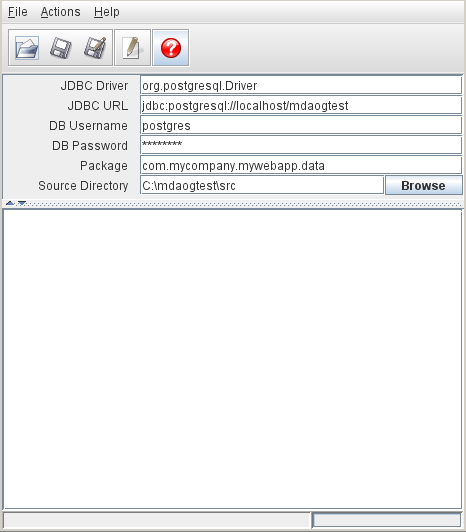
\includegraphics[width=0.65\textwidth]{figuras/mdaogMetal.png}
  \caption{Captura de pantalla de la interfaz de MDAOG}
  \label{fig:mdaog}
\end{figure}

Una \textbf{ventaja} de el uso de generadores de código es que no se agrega procesamiento extra a el programa, por ejemplo no hay por debajo un componente que se este encargando de realizar tareas si no que es el código generado el que directamente realiza estas tareas, como \textbf{desventaja} de los generadores de código es que siempre se esta trabajando sobre una misma plantilla, a menos claro que existen diferentes plantillas, a partir de la cual se genera el código, pero de todos modos siempre el código generado tendera a crear código de mas por que no es posible o viable (pensando en un auto-generador) estar ajustando la plantilla de acuerdo a las necesidades especificas de cada tabla o base de datos pues se pierde la gracia de este tipo de herramientas.
%
\section{Herramientas ORM}
Las herramientas ORM de \textit{Object-Relational Mapping} o mapeo objeto-relacional se encargan de eliminar de cierto modo la diferencia de paradigmas existente entre una aplicación que es orientada a objetos y un almacenamiento de datos que sigue un modelo relacional creando virtualmente una base de datos orientada a objetos sobre la base relacional, de este modo se eliminan muchas tareas extras relacionadas con el mapeo y además se adquiere beneficios extras al poder utilizar el paradigma POO sobre los datos.

Uno de los ejemplos mas conocidos de estas herramientas  es Hibernate, esta es una herramienta para la plataforma Java (y disponible también para .Net con el nombre de NHibernate) que facilita el mapeo de atributos entre una base de datos relacional tradicional y el modelo de objetos de una aplicación, mediante archivos declarativos (XML) o anotaciones en los beans\footnote{Los JavaBeans son un modelo de componentes para la construcción de aplicaciones en Java.} de las entidades que permiten establecer estas relaciones. Hibernate es una herramienta bastante poderosa una vez que se aprende a utilizarla, que termino convirtiéndose en un conjunto de herramientas relacionadas que brindan una solución bastante completa.
\begin{lstlisting}[title=Minimo ejemplo de Hibernate: guardando datos en la DB]
Session session = sessionFactory.openSession();
session.beginTransaction();
session.save( new Event( "Our very first event!", new Date() ) );
session.save( new Event( "A follow up event", new Date() ) );
session.getTransaction().commit();
session.close();
\end{lstlisting}
A diferencia de DAO, ORM trata específicamente el problema de uso de persistencia de datos con base de datos relacionales mientras que DAO en este sentido es mas generico pues considera otros tipos de soluciones para persistencia de datos y a diferencia de los generadores de código con los ORM no se genera código si no que se construye a medida con la herramienta. La única ventaja que se puede encontrar es que al ser una herramienta tan completa pueda ser demasiado para algunas situaciones, como dice el dicho popular seria como matar moscas con un cañón.
%
\section{Otras Soluciones}
Las diferentes soluciones existentes para lidiar con la abstracción de uso de las fuentes de datos se basan en técnicas o patrones de diseño preexistentes que brindan una base mejor fundamentada para el desarrollo de las mismas, como ultimo ejemplo de este tipo de soluciones podemos nombrar aquellas basadas en el patrón \textit{Active Record} en que un Objeto esta relacionado a una fila de una tabla por lo que una creación de un objeto equivale a crear una nueva fila en la tabla mediante una acción de guardar, lo mismo con las actualizaciones de datos de un objeto se reflejan en actualizaciones en la tabla. Un ejemplo de una herramienta que trabaja sobre \textit{Active Record} es activejdbc que puede ser encontrado en \href{http://code.google.com/p/activejdbc/}{code.google.com/p/activejdbc}, es una herramienta relativamente nueva que se publico por primera vez en el 2010 bajo la licencia Apache 2.0. Como  una caracteristica interesante de activejdbc es que no es necesario especificar el modelo de datos, este es inferido directamente desde la base de datos. En el ejemplo siguiente es suficiente que exista la siguiente tabla en la base de datos:
%
\begin{lstlisting}[title=Ejemplo de uso de activejdbc: tabla que debe existir en la BD]
CREATE TABLE people (
  id  int(11) NOT NULL auto_increment PRIMARY KEY, 
  name VARCHAR(56) NOT NULL, 
  last_name VARCHAR(56), 
  dob DATE, 
  graduation_date DATE, 
  created_at DATETIME, 
  updated_at DATETIME
  );
\end{lstlisting}
%
para que se pueda crear una nueva fila correspondiente a una persona \verb=person= en la tabla \verb=people= (plural de person) mediante las siguientes lineas de código: 
\begin{lstlisting}[title=Ejemplo de uso de activejdbc: creando una nueva fila en una tabla]
Person p = new Person();
p.set("name", "Marilyn");
p.set("last_name", "Monroe");
p.set("dob", "1935-12-06");
p.saveIt(); 
\end{lstlisting}
%

Como comentario final para cerrar este capitulo se quiere comentar que el espacio que quiere ocupar este proyecto es el de una herramienta que sea sencilla de utilizar y con mínimas dependencias de librerías externas y con la menor carga posible en el uso de recursos, se usara el patrón DAO como base de diseño pero no de una manera completa puesto que se requeriría crear una suerte de generador de código para cubrir completamente los requerimientos de DAO, en vez de eso se brindaran las herramientas para que la implementación de DAO resulte sencilla.
